\section{指数族}
\label{sec:dfam-exponential}

把Bernoulli、Poisson和高斯的概率公式取对数，会看到同一个结构。Bernoulli分布的对数质量是$x\ln\frac{p}{1-p}+\ln(1-p)$，Poisson分布是$x\ln\lambda-\lambda-\ln x!$，高斯分布是$x$与$x^{2}$的线性组合再加常数。三者都是“若干个统计量的线性组合，加上只依赖参数的归一化项，再加上只依赖$x$的项”。改变参数，就是改变给每个统计量的指数权重。

这一节先把这种形式写准，区分哪些对象固定、哪些随参数变化；再确定参数能取哪些值；然后看归一化项的导数怎样给出矩；最后把指数权重与它产生的均值对应起来。

\subsection{指数形式}
\label{sec:dfam-exponential-form}

\begin{definition}[指数族]
\label{def:dfam-exponential-family}
设$\nu$是$\mathcal{X}$上的$\sigma$有限测度，$h:\mathcal{X}\to[0,\infty)$与$\bm{T}:\mathcal{X}\to\mathbb{R}^{k}$可测，$\nu(\{h>0\})>0$。对使
\begin{equation}
  Z(\bm{\theta})=\int_{\mathcal{X}}h(x)\,\mathrm{e}^{\langle\bm{\theta},\bm{T}(x)\rangle}\,\nu(\mathrm{d}x)<\infty
  \label{eq:dfam-partition}
\end{equation}
的$\bm{\theta}\in\mathbb{R}^{k}$，令$A(\bm{\theta})=\ln Z(\bm{\theta})$，并以
\begin{equation}
  p_{\bm{\theta}}(x)=h(x)\exp\bigl(\langle\bm{\theta},\bm{T}(x)\rangle-A(\bm{\theta})\bigr)
  \label{eq:dfam-exponential-family}
\end{equation}
为相对$\nu$的密度定义$P_{\bm{\theta}}$。这样得到的分布族称为\term{指数族}（exponential family）。$\bm{T}$称为\term{自然统计量}（natural statistic），$\bm{\theta}$称为\term{自然参数}（natural parameter），$Z$与$A$分别称为\term{配分函数}（partition function）与\term{对数配分函数}（log-partition function）。
\end{definition}

式~\eqref{eq:dfam-exponential-family}中有三样东西是事先固定的：参考测度$\nu$、函数$h$和统计量$\bm{T}$。$h$与$\nu$只以乘积$h(x)\nu(\mathrm{d}x)$的形式出现，这个乘积称为\term{基准测度}（base measure），它决定哪些$x$可能出现，以及在不加任何指数权重时质量怎样分布。随参数变化的只有$\bm{\theta}$；$A(\bm{\theta})$不是另一个可以自由选择的量，它由归一化唯一确定，保证$p_{\bm{\theta}}$积分为$1$。

由式~\eqref{eq:dfam-exponential-family}，$p_{\bm{\theta}}(x)>0$当且仅当$h(x)>0$。所以指数族的所有成员有共同的支撑$\{h>0\}$，参数只改变支撑上质量的相对多少，不能把质量挪到$h$为零的地方。$\operatorname{Unif}(0,\theta)$的支撑随$\theta$变化，它就不能写成任何指数族。

\paragraph{三个分布的指数形式}
Bernoulli分布取$\nu$为$\{0,1\}$上的计数测度，
\[
  p^{x}(1-p)^{1-x}=\exp\Bigl(x\ln\frac{p}{1-p}+\ln(1-p)\Bigr).
\]
对照式~\eqref{eq:dfam-exponential-family}，$h=1$，$T(x)=x$，自然参数$\theta=\ln\frac{p}{1-p}$，即$p=\mathrm{e}^{\theta}/(1+\mathrm{e}^{\theta})$，再由$-A(\theta)=\ln(1-p)$得
\[
  A(\theta)=\ln(1+\mathrm{e}^{\theta}).
\]

Poisson分布取$\nu$为$\{0,1,2,\dots\}$上的计数测度，
\[
  \mathrm{e}^{-\lambda}\frac{\lambda^{x}}{x!}=\frac{1}{x!}\exp(x\ln\lambda-\lambda),
\]
所以$h(x)=1/x!$，$T(x)=x$，$\theta=\ln\lambda$，$A(\theta)=\mathrm{e}^{\theta}$。

高斯分布$\mathcal{N}(m,s^{2})$取$\nu$为Lebesgue测度，把指数中的平方展开：
\[
  \frac{1}{\sqrt{2\pi s^{2}}}\mathrm{e}^{-\frac{(x-m)^{2}}{2s^{2}}}=\frac{1}{\sqrt{2\pi}}\exp\Bigl(\frac{m}{s^{2}}x-\frac{1}{2s^{2}}x^{2}-\frac{m^{2}}{2s^{2}}-\ln s\Bigr).
\]
于是$h=1/\sqrt{2\pi}$，$\bm{T}(x)=(x,x^{2})$，自然参数是
\begin{equation}
  \bm{\theta}=(\theta_1,\theta_2)=\Bigl(\frac{m}{s^{2}},\ -\frac{1}{2s^{2}}\Bigr).
  \label{eq:dfam-gaussian-natural}
\end{equation}
反解得$s^{2}=-1/(2\theta_2)$，$m=-\theta_1/(2\theta_2)$，代入$\frac{m^{2}}{2s^{2}}+\ln s$，得到
\begin{equation}
  A(\bm{\theta})=-\frac{\theta_1^{2}}{4\theta_2}-\frac12\ln(-2\theta_2).
  \label{eq:dfam-gaussian-log-partition}
\end{equation}

\paragraph{同一个分布的不同写法}
指数形式不是唯一的。把高斯的统计量换成$\bm{T}'(x)=(x,-x^{2}/2)$，自然参数就变成$(m/s^{2},\ 1/s^{2})$；常数$1/\sqrt{2\pi}$也可以从$h$移进$A$。一般地，统计量作可逆线性变换$\bm{T}'=\bm{L}\bm{T}$，自然参数就作相应的变换$\bm{\theta}'=\bm{L}^{-\top}\bm{\theta}$，于是
\[
  \langle\bm{\theta}',\bm{T}'\rangle=\bm{\theta}^{\top}\bm{L}^{-1}\bm{L}\bm{T}=\langle\bm{\theta},\bm{T}\rangle ,
\]
指数不变，分布族也不变。

所以“自然参数”是相对于选定的$\bm{T}$与$h\nu$而言的，不能把密度公式里出现的任意参数都叫作自然参数。高斯族的均值$m$在式~\eqref{eq:dfam-gaussian-natural}中与$s^{2}$纠缠在一起，又出现在$A$里，它不是这组表示下的自然参数。但若只看方差固定为$1$的子族$\{\mathcal{N}(m,1)\}$，取$h=\varphi$、$T(x)=x$，则
\[
  \varphi(x-m)=\varphi(x)\exp\bigl(mx-\tfrac12m^{2}\bigr),
\]
$m$恰好是自然参数，$A(m)=m^{2}/2$。同一个数字是否是自然参数，取决于整个表示。

写法还可能带来冗余。Bernoulli分布也可以写成
\[
  p^{x}(1-p)^{1-x}=\exp\bigl(\theta_0\mathbf{1}_{\{x=0\}}+\theta_1\mathbf{1}_{\{x=1\}}\bigr),\qquad(\theta_0,\theta_1)=(\ln(1-p),\ln p).
\]
两个统计量之和恒为$1$，把$(\theta_0,\theta_1)$同时加上同一个常数，归一化后分布不变。这种冗余与第~\ref{sec:dfam-identifiability}节的重复参数是同一回事，后面两小节会精确地描述它。

\subsection{自然参数域}
\label{sec:dfam-natural-domain}

式~\eqref{eq:dfam-exponential-family}只在$Z(\bm{\theta})$有限且为正时才定义了概率分布。被积函数在$\{h>0\}$上为正，而$\nu(\{h>0\})>0$，所以$Z(\bm{\theta})>0$总成立；问题只在于是否有限。

\begin{definition}[自然参数域]
\label{def:dfam-natural-domain}
集合
\begin{equation}
  \Theta=\{\bm{\theta}\in\mathbb{R}^{k}:Z(\bm{\theta})<\infty\}
  \label{eq:dfam-natural-domain}
\end{equation}
称为指数族的\term{自然参数域}（natural parameter space）。若$\Theta$是$\mathbb{R}^{k}$中的开集，称这个指数族是\term{正则指数族}（regular exponential family）。
\end{definition}

$\Theta$以外的$\bm{\theta}$给出的表达式$h\,\mathrm{e}^{\langle\bm{\theta},\bm{T}\rangle}$不能归一化，它只是一个形式表达式，不是概率分布。例如在$(0,\infty)$上取$h=1$、$T(x)=x$，$\int_0^\infty\mathrm{e}^{\theta x}\,\mathrm{d}x$在$\theta<0$时等于$-1/\theta$，在$\theta\geq0$时发散。所以$\Theta=(-\infty,0)$，$\theta=-\lambda$对应$\operatorname{Exp}(\lambda)$，$A(\theta)=-\ln(-\theta)$。

\begin{lemma}[自然参数域的凸性]
\label{lem:dfam-domain-convex}
$\Theta$是凸集，$A$是$\Theta$上的凸函数。
\end{lemma}

\begin{proof}
设$\bm{\theta},\bm{\theta}'\in\Theta$，$0<\lambda<1$。被积函数可以拆成两个幂的乘积：
\[
  \mathrm{e}^{\langle\lambda\bm{\theta}+(1-\lambda)\bm{\theta}',\bm{T}\rangle}=\bigl(\mathrm{e}^{\langle\bm{\theta},\bm{T}\rangle}\bigr)^{\lambda}\bigl(\mathrm{e}^{\langle\bm{\theta}',\bm{T}\rangle}\bigr)^{1-\lambda}.
\]
对测度$h\nu$用指数为$1/\lambda$与$1/(1-\lambda)$的Hölder不等式（见\BookChapterRef{chap:function-normed-spaces}{卷四第11章“赋范空间”}），
\[
  Z\bigl(\lambda\bm{\theta}+(1-\lambda)\bm{\theta}'\bigr)\leq Z(\bm{\theta})^{\lambda}Z(\bm{\theta}')^{1-\lambda}<\infty .
\]
所以$\lambda\bm{\theta}+(1-\lambda)\bm{\theta}'\in\Theta$。两边取对数，得到
\[
  A\bigl(\lambda\bm{\theta}+(1-\lambda)\bm{\theta}'\bigr)\leq\lambda A(\bm{\theta})+(1-\lambda)A(\bm{\theta}') .
\]
\end{proof}

\paragraph{几个参数域}
Bernoulli与Poisson的配分和对任何$\theta$都有限，$\Theta=\mathbb{R}$。高斯族的配分积分是
\[
  Z(\bm{\theta})=\frac{1}{\sqrt{2\pi}}\int_{-\infty}^{\infty}\mathrm{e}^{\theta_1x+\theta_2x^{2}}\,\mathrm{d}x ,
\]
它在$\theta_2<0$时有限；$\theta_2=0$时被积函数是$\mathrm{e}^{\theta_1x}$，在某一侧不衰减；$\theta_2>0$时在两侧都发散。所以$\Theta=\{(\theta_1,\theta_2):\theta_2<0\}$是开半平面，高斯族是正则的。

自然参数域不一定是开的。在$(0,\infty)$上取$h(x)=(1+x)^{-2}$、$T(x)=x$，
\[
  Z(\theta)=\int_0^\infty\frac{\mathrm{e}^{\theta x}}{(1+x)^{2}}\,\mathrm{d}x .
\]
$\theta>0$时被积函数趋于无穷，积分发散；$\theta\leq0$时被积函数不超过$(1+x)^{-2}$，积分有限，且$Z(0)=1$。所以$\Theta=(-\infty,0]$，边界点$0$属于参数域，它对应的分布就是密度$(1+x)^{-2}$。这个分布的均值是$\int_0^\infty x(1+x)^{-2}\,\mathrm{d}x=\infty$。

图~\ref{fig:dfam-natural-domain}比较这两个一维的例子。指数分布族的$A(\theta)$在$\theta\uparrow0$时趋于无穷，参数域在$0$处断开；第二个族的$A(\theta)$在$0$处取有限值$0$，但均值$\mathbb{E}_\theta[X]$在$\theta\uparrow0$时趋于无穷，曲线在边界处变得竖直。边界点属于参数域，并不意味着那里的分布与内部一样好用：它的均值已经不存在了，下一小节的导数公式在那里不成立。

\begin{BookInlineFigure}
  \centering
  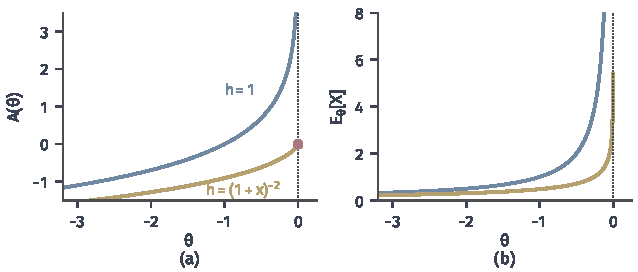
\includegraphics[width=108mm]{figures/07-probability/04-distribution-analysis/matplotlib/dfam-natural-domain/figure.pdf}
  \caption{两个一维指数族的自然参数域，$T(x)=x$，$x>0$。蓝：$h=1$（指数分布族），$\Theta=(-\infty,0)$；黄：$h(x)=(1+x)^{-2}$，$\Theta=(-\infty,0]$，红点是属于参数域的边界点$\theta=0$。(a)对数配分函数$A(\theta)$。(b)均值$\mathbb{E}_\theta[X]$，两者在$\theta\uparrow0$时都趋于无穷。黄线由数值积分得到。}
  \label{fig:dfam-natural-domain}
\end{BookInlineFigure}

\paragraph{退化的极限}
参数趋于无穷时，分布可能趋于族外的分布。在$\{0,1,2\}$上取计数测度、$h=1$、$T(x)=x$，得到一个单参数指数族
\begin{equation}
  p_\theta(x)=\frac{\mathrm{e}^{\theta x}}{1+\mathrm{e}^{\theta}+\mathrm{e}^{2\theta}},\qquad x=0,1,2,\quad\theta\in\mathbb{R}.
  \label{eq:dfam-tilt}
\end{equation}
它从均匀表出发，按$\mathrm{e}^{\theta x}$给较大的点数加权：$\theta=0$时是均匀表，$\theta=\ln2$时权重为$1,2,4$，
\[
  p_{\ln2}=\bigl(\tfrac17,\ \tfrac27,\ \tfrac47\bigr).
\]
$\theta\to+\infty$时，分子分母同除以$\mathrm{e}^{2\theta}$，$p_\theta(2)\to1$，分布趋于点质量$\delta_2$；$\theta\to-\infty$时趋于$\delta_0$。

但$\delta_2$不等于任何$p_\theta$，因为每个$p_\theta$在三个点上都为正。图~\ref{fig:dfam-tilt-simplex}把这个族画在第~\ref{sec:dfam-candidates}节的三角形中：它是穿过内部的一条曲线，两端无限接近顶点而不到达。族的闭包含有边界上的分布，而这些分布不能用有限的自然参数表示。

\begin{BookInlineFigure}
  \centering
  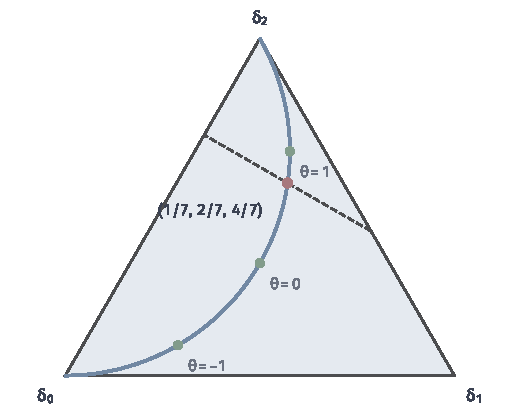
\includegraphics[width=88mm]{figures/07-probability/04-distribution-analysis/matplotlib/dfam-tilt-simplex/figure.pdf}
  \caption{式~\eqref{eq:dfam-tilt}的单参数指数族在三角形$\Delta_2$中的轨迹（蓝线），$\theta$从$-6$到$6$。绿点依次是$\theta=-1,0,1$，红点是$\theta=\ln2$对应的$(\frac17,\frac27,\frac47)$；曲线两端趋于顶点$\delta_0$与$\delta_2$，但不到达。深灰虚线是满足$\mathbb{E}_P[X]=\frac{10}{7}$的全部概率表，它与曲线只交于红点。}
  \label{fig:dfam-tilt-simplex}
\end{BookInlineFigure}

\subsection{配分函数的导数}
\label{sec:dfam-partition-derivatives}

对数配分函数原本只是为归一化而设，但它把整个族的矩都存了起来。对式~\eqref{eq:dfam-partition}关于$\theta_j$求导，形式上会在积分号内落下一个因子$T_j(x)$，这正是$T_j$的期望。下面的定理说明，在参数域内部这个形式计算是合法的。

\begin{theorem}[对数配分函数的导数]
\label{thm:dfam-log-partition-derivatives}
设$\bm{\theta}$是$\Theta$的内点。则在$P_{\bm{\theta}}$下$\bm{T}$的各分量有任意阶矩，$A$在$\bm{\theta}$处二阶可微，且
\begin{equation}
  \nabla A(\bm{\theta})=\mathbb{E}_{\bm{\theta}}[\bm{T}],\qquad\nabla^{2}A(\bm{\theta})=\operatorname{Cov}_{\bm{\theta}}(\bm{T}).
  \label{eq:dfam-log-partition-derivatives}
\end{equation}
\end{theorem}

\begin{proof}
取$\varepsilon>0$，使立方体$K=\bm{\theta}+[-2\varepsilon,2\varepsilon]^{k}$含于$\Theta$。函数$\bm{\eta}\mapsto\mathrm{e}^{\langle\bm{\eta},\bm{T}(x)\rangle}$是凸的，它在立方体$K$上的最大值在某个顶点处取到，所以对$\bm{\eta}\in K$，
\[
  \mathrm{e}^{\langle\bm{\eta},\bm{T}(x)\rangle}\leq G(x)=\sum_{\bm{v}}\mathrm{e}^{\langle\bm{v},\bm{T}(x)\rangle},
\]
其中$\bm{v}$取遍$K$的$2^{k}$个顶点。每个顶点都在$\Theta$中，所以$G$对$h\nu$可积。

再把统计量的多项式因子吸收进指数。由$\mathrm{e}^{s}\geq s$与$\mathrm{e}^{s}\geq s^{2}/2$（$s\geq0$），对实数$t$有
\[
  \lvert t\rvert\leq\frac{\mathrm{e}^{\varepsilon t}+\mathrm{e}^{-\varepsilon t}}{\varepsilon},\qquad t^{2}\leq\frac{2(\mathrm{e}^{\varepsilon t}+\mathrm{e}^{-\varepsilon t})}{\varepsilon^{2}} .
\]
设$\bm{\theta}'\in\bm{\theta}+[-\varepsilon,\varepsilon]^{k}$，则$\bm{\theta}'\pm\varepsilon\bm{e}_j\in K$。取$t=T_j(x)$，第二个不等式给出
\[
  T_j(x)^{2}\,\mathrm{e}^{\langle\bm{\theta}',\bm{T}(x)\rangle}\leq\frac{2}{\varepsilon^{2}}\bigl(\mathrm{e}^{\langle\bm{\theta}'+\varepsilon\bm{e}_j,\bm{T}\rangle}+\mathrm{e}^{\langle\bm{\theta}'-\varepsilon\bm{e}_j,\bm{T}\rangle}\bigr)\leq\frac{4}{\varepsilon^{2}}G(x).
\]
用第一个不等式同样得到
\[
  \lvert T_j\rvert\,\mathrm{e}^{\langle\bm{\theta}',\bm{T}\rangle}\leq\frac{2}{\varepsilon}G ,
\]
而由$\lvert T_iT_j\rvert\leq(T_i^{2}+T_j^{2})/2$，交叉项也被$4G/\varepsilon^{2}$控制。对更高的$r$次幂，由$\mathrm{e}^{s}\geq s^{r}/r!$（$s\geq0$）同样把$\lvert T_j\rvert^{r}$吸收进指数，得到任意阶矩有限。

有了与$\bm{\theta}'$无关的可积控制函数，由中值定理与控制收敛定理，可以在积分号下对$Z$求一阶和二阶偏导数（见\BookChapterRef{chap:integration}{卷四第6章“积分”}）：
\[
  \partial_jZ(\bm{\theta})=\int T_j\,h\,\mathrm{e}^{\langle\bm{\theta},\bm{T}\rangle}\,\mathrm{d}\nu,\qquad\partial_i\partial_jZ(\bm{\theta})=\int T_iT_j\,h\,\mathrm{e}^{\langle\bm{\theta},\bm{T}\rangle}\,\mathrm{d}\nu ,
\]
并且这些偏导数在$\bm{\theta}$附近连续。

除以$Z(\bm{\theta})$，就是$P_{\bm{\theta}}$下的期望：
\[
  \frac{\partial_jZ}{Z}=\mathbb{E}_{\bm{\theta}}[T_j],\qquad\frac{\partial_i\partial_jZ}{Z}=\mathbb{E}_{\bm{\theta}}[T_iT_j].
\]
由$A=\ln Z$，一阶偏导数是
\[
  \partial_jA=\frac{\partial_jZ}{Z}=\mathbb{E}_{\bm{\theta}}[T_j].
\]
再求一次导，
\[
  \partial_i\partial_jA=\frac{\partial_i\partial_jZ}{Z}-\frac{\partial_iZ\,\partial_jZ}{Z^{2}}=\mathbb{E}_{\bm{\theta}}[T_iT_j]-\mathbb{E}_{\bm{\theta}}[T_i]\,\mathbb{E}_{\bm{\theta}}[T_j].
\]
这就是$\operatorname{Cov}_{\bm{\theta}}(T_i,T_j)$。
\end{proof}

定理只对内点成立。上一小节的边界点$\theta=0$处，$\mathbb{E}_0[X]=\infty$，一阶导数公式已经失去意义。

\paragraph{例子中的导数}
Bernoulli族$A(\theta)=\ln(1+\mathrm{e}^{\theta})$，求导得
\[
  A'(\theta)=\frac{\mathrm{e}^{\theta}}{1+\mathrm{e}^{\theta}}=p,\qquad A''(\theta)=p(1-p),
\]
正是$\operatorname{Bern}(p)$的均值与方差。Poisson族$A(\theta)=\mathrm{e}^{\theta}=\lambda$，一阶、二阶导数都等于$\lambda$，均值与方差相等。

高斯族对式~\eqref{eq:dfam-gaussian-log-partition}求偏导，再用$m=-\theta_1/(2\theta_2)$与$s^{2}=-1/(2\theta_2)$换回去，
\[
  \frac{\partial A}{\partial\theta_1}=-\frac{\theta_1}{2\theta_2}=m,\qquad\frac{\partial A}{\partial\theta_2}=\frac{\theta_1^{2}}{4\theta_2^{2}}-\frac{1}{2\theta_2}=m^{2}+s^{2}.
\]
这正是$\mathbb{E}[X]$与$\mathbb{E}[X^{2}]$，与$\bm{T}=(x,x^{2})$对应。

对式~\eqref{eq:dfam-tilt}的族，对数配分函数是
\[
  A(\theta)=\ln\bigl(1+\mathrm{e}^{\theta}+\mathrm{e}^{2\theta}\bigr).
\]
在$\theta=\ln2$处，$\mathrm{e}^{\theta}=2$，
\[
  A(\ln2)=\ln7,\qquad A'(\ln2)=\frac{2+2\cdot4}{7}=\frac{10}{7}.
\]
再算二阶矩$\mathbb{E}[X^{2}]=(2+4\cdot4)/7=18/7$，于是
\[
  A''(\ln2)=\frac{18}{7}-\Bigl(\frac{10}{7}\Bigr)^{2}=\frac{26}{49}\approx0.531 .
\]
图~\ref{fig:dfam-log-partition}(a)中，红点处切线的斜率$10/7$就是这个分布的均值；(b)画出均值$A'(\theta)$与方差$A''(\theta)$随$\theta$的变化：均值从$0$单调升到$2$，方差在均值经过$1$时最大，在两端趋于零。

\begin{BookInlineFigure}
  \centering
  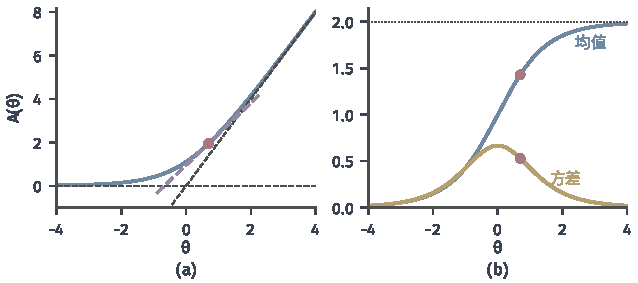
\includegraphics[width=108mm]{figures/07-probability/04-distribution-analysis/matplotlib/dfam-log-partition/figure.pdf}
  \caption{式~\eqref{eq:dfam-tilt}的对数配分函数。(a)$A(\theta)=\ln(1+\mathrm{e}^{\theta}+\mathrm{e}^{2\theta})$（蓝），红点$\theta=\ln2$处的切线（紫色虚线）斜率为$10/7$；两条深灰虚线是渐近线$y=0$与$y=2\theta$。(b)均值$A'(\theta)$（蓝）与方差$A''(\theta)$（黄），红点为$(\ln2,10/7)$与$(\ln2,26/49)$。}
  \label{fig:dfam-log-partition}
\end{BookInlineFigure}

\paragraph{累积量}
导数还能继续求下去。对$\bm{\theta}\in\Theta$与使$\bm{\theta}+\bm{t}\in\Theta$的$\bm{t}$，
\begin{equation}
  \ln\mathbb{E}_{\bm{\theta}}\bigl[\mathrm{e}^{\langle\bm{t},\bm{T}\rangle}\bigr]=\ln\frac{Z(\bm{\theta}+\bm{t})}{Z(\bm{\theta})}=A(\bm{\theta}+\bm{t})-A(\bm{\theta}).
  \label{eq:dfam-cumulant}
\end{equation}
左边是$\bm{T}$的矩母函数的对数，称为\term{累积量生成函数}（cumulant generating function）。式~\eqref{eq:dfam-cumulant}说明，在一个内点处，它就是把$A$平移到原点。$\bm{T}$在$P_{\bm{\theta}}$下的全部高阶矩信息，都由$A$在$\bm{\theta}$附近的形状给出。

\paragraph{凸性与仿射冗余}
由式~\eqref{eq:dfam-log-partition-derivatives}，对任意$\bm{a}\in\mathbb{R}^{k}$，
\[
  \bm{a}^{\top}\nabla^{2}A(\bm{\theta})\,\bm{a}=\operatorname{Var}_{\bm{\theta}}\bigl(\langle\bm{a},\bm{T}\rangle\bigr)\geq0 ,
\]
Hessian半正定，与引理~\ref{lem:dfam-domain-convex}的凸性相符。等号成立当且仅当$\langle\bm{a},\bm{T}\rangle$在$P_{\bm{\theta}}$下几乎必然为常数。

$P_{\bm{\theta}}$的密度在$\{h>0\}$上为正，所以$P_{\bm{\theta}}$与基准测度$h\nu$有相同的零测集，“$P_{\bm{\theta}}$下几乎必然”就是“$h\nu$下几乎处处”，与$\bm{\theta}$无关。于是Hessian在某个内点退化，当且仅当存在$\bm{a}\neq\bm{0}$与常数$c$，使
\begin{equation}
  \langle\bm{a},\bm{T}(x)\rangle=c\qquad\text{对}h\nu\text{几乎所有}x ,
  \label{eq:dfam-affine-redundancy}
\end{equation}
而这时它在所有内点处同时退化。式~\eqref{eq:dfam-affine-redundancy}说的是统计量之间有仿射关系，有一个分量是多余的。

第~\ref{sec:dfam-exponential-form}节Bernoulli的冗余写法正是如此：两个示性统计量满足$T_0+T_1=1$，取$\bm{a}=(1,1)$、$c=1$。这时
\[
  A(\bm{\theta})=\ln(\mathrm{e}^{\theta_0}+\mathrm{e}^{\theta_1}),\qquad A\bigl(\bm{\theta}+c'(1,1)\bigr)=A(\bm{\theta})+c',
\]
$A$沿$(1,1)$方向是线性的，不是严格凸的；而分布只依赖$\theta_1-\theta_0=\ln\frac{p}{1-p}$，沿这个方向完全不变。图~\ref{fig:dfam-overcomplete}画出这一点。

\begin{BookInlineFigure}
  \centering
  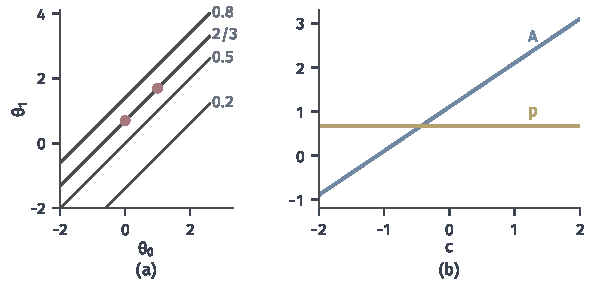
\includegraphics[width=100mm]{figures/07-probability/04-distribution-analysis/matplotlib/dfam-overcomplete/figure.pdf}
  \caption{Bernoulli族的冗余表示$\bm{T}=(\mathbf{1}_{\{x=0\}},\mathbf{1}_{\{x=1\}})$。(a)$(\theta_0,\theta_1)$平面中，分布相同的参数构成平行于$(1,1)$的直线（深灰），标注为对应的$p$；红点$(0,\ln2)$与$(1,1+\ln2)$都给出$p=\frac23$。(b)沿红点所在直线$\bm{\theta}=(0,\ln2)+c(1,1)$，$A$随$c$线性增长（蓝），而$p$保持$\frac23$（黄）。}
  \label{fig:dfam-overcomplete}
\end{BookInlineFigure}

\subsection{自然参数与均值参数}
\label{sec:dfam-natural-mean}

上一小节表明，Hessian退化与参数冗余是同一个现象。把统计量中多余的分量去掉，参数就不再冗余，而$\nabla A$给出的均值成为另一套可以替代自然参数的坐标。

\begin{definition}[最小表示与均值参数]
\label{def:dfam-minimal}
若不存在$\bm{a}\neq\bm{0}$与常数$c$使式~\eqref{eq:dfam-affine-redundancy}成立，则称指数族的这个表示是\term{最小表示}（minimal representation）。对$\bm{\theta}\in\Theta$，若$\mathbb{E}_{\bm{\theta}}[\bm{T}]$存在，称
\begin{equation}
  \bm{m}(\bm{\theta})=\mathbb{E}_{\bm{\theta}}[\bm{T}]
  \label{eq:dfam-mean-parameter}
\end{equation}
为$P_{\bm{\theta}}$的\term{均值参数}（mean parameter），$\bm{\theta}\mapsto\bm{m}(\bm{\theta})$称为\term{均值映射}（mean map）。
\end{definition}

在正则族中，每个$\bm{\theta}$都是内点，由定理~\ref{thm:dfam-log-partition-derivatives}，均值映射就是$\nabla A$。

\begin{theorem}[自然参数与均值参数的对应]
\label{thm:dfam-natural-mean}
设指数族采用最小表示。
\begin{enumerate}
  \item 参数化$\bm{\theta}\mapsto P_{\bm{\theta}}$在$\Theta$上可辨识。反之，若表示不是最小的，则参数化不可辨识。
  \item 若族还是正则的，则均值映射$\bm{m}=\nabla A$在$\Theta$上是单射，其Jacobian矩阵$\nabla^{2}A(\bm{\theta})$正定；像集$\mathcal{M}^{\circ}=\nabla A(\Theta)$是开集，逆映射$\mathcal{M}^{\circ}\to\Theta$连续可微。
  \item 在第二部分的条件下，若$\bm{a}\neq\bm{0}$且$\langle\bm{a},\bm{T}\rangle\leq c$对$h\nu$几乎所有$x$成立，则对每个$\bm{m}\in\mathcal{M}^{\circ}$有$\langle\bm{a},\bm{m}\rangle<c$。
\end{enumerate}
\end{theorem}

\begin{proof}
第一部分。设$P_{\bm{\theta}}=P_{\bm{\theta}'}$，则两个密度在$h\nu$下几乎处处相等。在$\{h>0\}$上取对数，得到
\[
  \langle\bm{\theta}-\bm{\theta}',\bm{T}(x)\rangle=A(\bm{\theta})-A(\bm{\theta}')\qquad\text{对}h\nu\text{几乎所有}x .
\]
这是形如式~\eqref{eq:dfam-affine-redundancy}的关系，$\bm{a}=\bm{\theta}-\bm{\theta}'$。最小表示排除了$\bm{a}\neq\bm{0}$，所以$\bm{\theta}=\bm{\theta}'$。

反之，若式~\eqref{eq:dfam-affine-redundancy}对某个$\bm{a}\neq\bm{0}$成立，取$\bm{\theta}\in\Theta$与$t\neq0$。在$h\nu$下几乎处处有
\[
  \mathrm{e}^{\langle\bm{\theta}+t\bm{a},\bm{T}\rangle}=\mathrm{e}^{tc}\,\mathrm{e}^{\langle\bm{\theta},\bm{T}\rangle},
\]
两边积分，
\[
  Z(\bm{\theta}+t\bm{a})=\mathrm{e}^{tc}Z(\bm{\theta})<\infty ,
\]
所以$\bm{\theta}+t\bm{a}\in\Theta$。两个密度中的因子$\mathrm{e}^{tc}$被归一化抵消，$P_{\bm{\theta}+t\bm{a}}=P_{\bm{\theta}}$，参数化不可辨识。

第二部分。由上一小节，最小表示下$\nabla^{2}A(\bm{\theta})$对每个$\bm{\theta}\in\Theta$正定。设$\bm{\theta}\neq\bm{\theta}'$，令$g(t)=A(\bm{\theta}'+t(\bm{\theta}-\bm{\theta}'))$，$t\in[0,1]$。$\Theta$凸，线段在$\Theta$内，
\[
  g''(t)=(\bm{\theta}-\bm{\theta}')^{\top}\nabla^{2}A\,(\bm{\theta}-\bm{\theta}')>0 ,
\]
所以$g'$严格递增，$g'(1)>g'(0)$，即
\[
  \bigl\langle\nabla A(\bm{\theta})-\nabla A(\bm{\theta}'),\ \bm{\theta}-\bm{\theta}'\bigr\rangle>0 .
\]
这说明$\nabla A(\bm{\theta})\neq\nabla A(\bm{\theta}')$，均值映射是单射。定理~\ref{thm:dfam-log-partition-derivatives}的证明给出$\nabla A$连续可微，Jacobian矩阵$\nabla^{2}A$正定因而可逆。由反函数定理（见\BookChapterRef{chap:implicit-inverse-functions}{卷二第22章“隐函数与反函数”}），$\nabla A$把每个点的一个邻域连续可微地一一映到一个开集上，于是像集$\mathcal{M}^{\circ}$是开集；结合全局单射，这些局部逆拼成一个连续可微的全局逆。

第三部分。设$\bm{m}=\nabla A(\bm{\theta})$且$\langle\bm{a},\bm{m}\rangle=c$。则$c-\langle\bm{a},\bm{T}\rangle$在$P_{\bm{\theta}}$下几乎必然非负，期望为零，所以几乎必然为零，也就是在$h\nu$下几乎处处有$\langle\bm{a},\bm{T}\rangle=c$，与最小表示矛盾。而$\langle\bm{a},\bm{m}\rangle\leq c$由期望的保序得到，所以严格不等式成立。
\end{proof}

第三部分说的是：统计量的取值被一个半空间$\{\langle\bm{a},\bm{t}\rangle\leq c\}$围住时，族中任何分布的均值都严格落在半空间内部，碰不到边界。边界上的均值只能由把全部质量放在超平面$\{\langle\bm{a},\bm{t}\rangle=c\}$上的分布实现，而指数族的成员都与基准测度有相同的零测集，做不到这一点。

\paragraph{三个例子}
Bernoulli族是最小表示，均值参数就是$p$。所有$\{0,1\}$上分布的均值组成$[0,1]$，均值映射的像却只是$(0,1)$：端点$0$与$1$是$\delta_0$与$\delta_1$的均值，它们不在族中，与第三部分（取$\bm{a}=\pm1$）一致。

式~\eqref{eq:dfam-tilt}的族中，均值映射$A'$把$\mathbb{R}$一一映到$(0,2)$。给定均值，可以反解自然参数。设均值为$10/7$，记$r=\mathrm{e}^{\theta}$，方程$A'(\theta)=10/7$是
\[
  \frac{r+2r^{2}}{1+r+r^{2}}=\frac{10}{7}.
\]
去分母并整理，得到
\[
  4r^{2}-3r-10=0 .
\]
它的正根是$r=(3+13)/8=2$（另一根$-5/4$为负，舍去），所以$\theta=\ln2$，回到$(\tfrac17,\tfrac27,\tfrac47)$。图~\ref{fig:dfam-tilt-simplex}中，这就是深灰虚线与曲线的交点。

高斯族中，均值参数是$(\mathbb{E}[X],\mathbb{E}[X^{2}])=(m,m^{2}+s^{2})$。由$s^{2}>0$，像集是抛物线上方的开区域
\[
  \mathcal{M}^{\circ}=\{(\eta_1,\eta_2):\eta_2>\eta_1^{2}\}.
\]
抛物线$\eta_2=\eta_1^{2}$本身对应方差为零的点质量，也是一切实值分布的$(\mathbb{E}[X],\mathbb{E}[X^{2}])$可以达到、指数族却达不到的边界。逆映射是$m=\eta_1$、$s^{2}=\eta_2-\eta_1^{2}$，代入式~\eqref{eq:dfam-gaussian-natural}即回到自然参数。例如$\bm{\theta}=(1,-\tfrac12)$对应$\mathcal{N}(1,1)$，均值参数是$(1,2)$。图~\ref{fig:dfam-mean-map}画出这对坐标之间的对应。

\begin{BookInlineFigure}
  \centering
  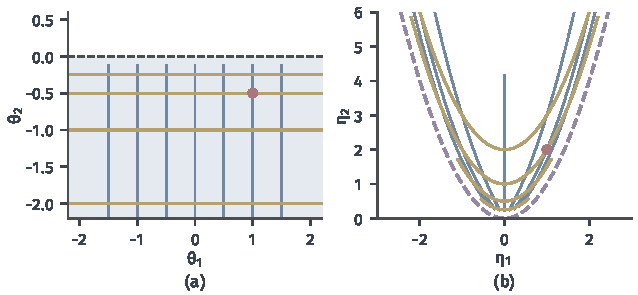
\includegraphics[width=108mm]{figures/07-probability/04-distribution-analysis/matplotlib/dfam-mean-map/figure.pdf}
  \caption{高斯族的自然参数与均值参数。(a)自然参数域是半平面$\theta_2<0$（浅蓝），画出直线族$\theta_1=$常数（蓝）与$\theta_2=$常数（黄）。(b)它们经$\nabla A$映到抛物线$\eta_2=\eta_1^{2}$（紫色虚线）上方的区域。红点是$\mathcal{N}(1,1)$：$\bm{\theta}=(1,-\frac12)$，$\bm{\eta}=(1,2)$。抛物线本身对应点质量，不在像中。}
  \label{fig:dfam-mean-map}
\end{BookInlineFigure}

\paragraph{对应的范围}
定理~\ref{thm:dfam-natural-mean}的坐标对应只在正则族的参数域与均值映射的像$\mathcal{M}^{\circ}$之间成立。它不覆盖可行均值的边界，也不覆盖非正则族的边界参数：第~\ref{sec:dfam-natural-domain}节中$h=(1+x)^{-2}$的族，边界点$\theta=0$在参数域中，那里却没有有限的均值参数。给定一个均值时是否存在族中的分布、存在时怎样求出对应的自然参数，以及在$\mathcal{M}^{\circ}$之外怎样处理，是第~\ref{chap:distribution-selection}章矩匹配的问题；两套坐标之间更细的几何关系由第~\ref{chap:information-geometry}章展开。
